\documentclass[10pt,twocolumn,twoside,czech,a4paper]{article}

\usepackage[czech]{babel}
\usepackage[utf8]{inputenc}
\usepackage{graphicx}
\usepackage{url}
\usepackage{hyperref}
\usepackage{wrapfig}
\usepackage{amsmath}

\usepackage{cite}

\pagestyle{headings}

\title{P2P Protokoly pro přenos souborů\thanks{Semestrální projekt v předmětu Metody inženýrské práce, ak. rok 2023/24, vedení: Ing. Richard Marko, PhD.}}

\author{Andrei Yakuta\\[2pt]
	{\small Slovenská technická univerzita v Bratislavě}\\
	{\small Fakulta informatiky a informačních technologií}\\
	{\small \texttt{xyakuta@stuba.sk}}
	}




\begin{document}

\maketitle

\begin{abstract}
\ldots
\end{abstract}



\section{Úvod}

P2P (Peer-to-Peer) protokoly pro přenos souborů představují způsob sdílení dat mezi uzly ve stejné síti bez nutnosti centrálního serveru.
Tento způsob sdílení dat umožňuje výrazné snížení nákladů na infrastrukturu, zatímco zajišťuje rychlý a spolehlivý přenos velkých souborů.
V mém projektu se zaměřím na analýzu různých P2P protokolů, jako jsou BitTorrent, eDonkey a Gnutella.

\begin{wrapfigure}{r}{0.35\textwidth}
	\centering
	
\includegraphics[width=0.5\textwidth]{logo.pdf}
\end{wrapfigure}

Hlavním cílem je porozumění architektuře těchto protokolů, mechanismům vyhledávání a sdílení souborů, a způsobům, jak tyto protokoly řeší problémy s bezpečností a soukromím.
Porovnám také P2P protokoly s tradičními client-server modely, abych diskutoval o výhodách a nevýhodách obou přístupů.
Důležitou součástí mé analýzy bude hodnocení různých implementací P2P protokolů a jejich dopad na výkon, škálovatelnost a odolnost proti chybám.
Dále se pokusím předvídat možný vývoj P2P technologií a zvážit jejich potenciální dopad na budoucí aplikace a služby v digitálním světě.


\begin{equation*}
	\begin{pmatrix}
	  1 & 2 & 3 & 4 \\
	  5 & 6 & 7 & 8 \\
	  9 & 10 & 11 & 12 \\
	  13 & 14 & 15 & 16 \\
	  17 & 18 & 19 & 20
	\end{pmatrix}
\end{equation*}


\begin{figure*}[h]
	\centering
	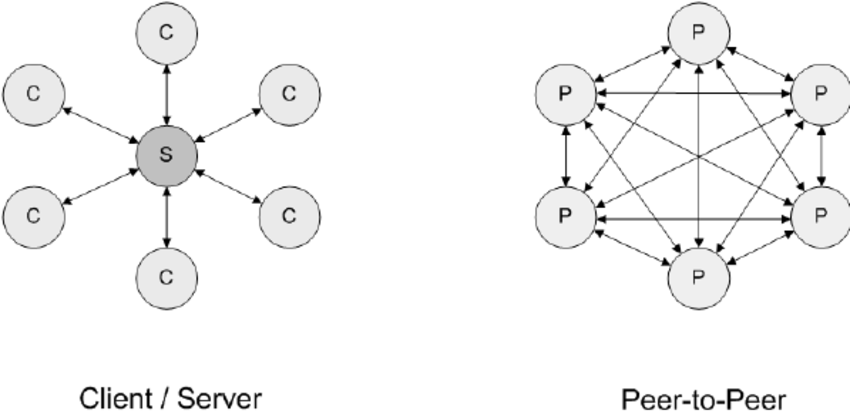
\includegraphics[width=1.0\textwidth]{client-server-vs-p2p.png}
\end{figure*}

\begin{equation*}
	\left\{n\right\}^{\infty}_{n=1}=\left\{1,2,3,4,5,6,7,8,9,10,11,12,13,14,15,16,17,18,19,20,21,\ldots\right\}
\end{equation*}	

\bibliography{literatura}
\bibliographystyle{plain} % prípadne alpha, abbrv alebo hociktorý iný
\end{document}
